\documentclass[12pt, a4paper, twoside]{book}
\usepackage[utf8]{inputenc} % Aceptar diferentes tipos de codificación de caracteres de entrada (en este caso usamos la codificación Unicode UTF-8)
%\usepackage{natbib}
\usepackage{listings}
\usepackage{eurosym}
\usepackage[spanish]{babel}
\usepackage{titlesec}
\usepackage{graphicx} % Soporte aumentado para gráficos 
\usepackage{float}
\usepackage{hyperref} % Para manejar referencias cruzadas. P.ej. añadir hiperenlaces al índice
\usepackage{caption}
\usepackage{setspace}
\usepackage{color}
\usepackage[a4paper, top=3.5cm, bottom=3.5cm, left=3cm, right=3cm]{geometry}
\spacing{1.5}
\setcounter{secnumdepth}{4}
\setlength{\parindent}{12pt}
\titleformat{\paragraph}
{\normalfont\normalsize\bfseries}{\theparagraph}{1em}{}
\titlespacing*{\paragraph}
{0pt}{3.25ex plus 1ex minus .2ex}{1.5ex plus .2ex}

%\usepackage{inconsolata}
%
%\usepackage[T1]{fontenc}
%
%\definecolor{pblue}{rgb}{0.13,0.13,1}
%\definecolor{pgreen}{rgb}{0,0.5,0}
%\definecolor{pred}{rgb}{0.9,0,0}
%\definecolor{pgrey}{rgb}{0.46,0.45,0.48}
%
%\lstset{language=Java,
%	showspaces=false,
%	showtabs=false,
%	breaklines=true,
%	showstringspaces=false,
%	breakatwhitespace=true,
%	commentstyle=\color{pgreen},
%	keywordstyle=\color{pblue},
%	stringstyle=\color{pred},
%	basicstyle=\ttfamily,
%	moredelim=[il][\textcolor{pgrey}]{$$},
%	moredelim=[is][\textolor{pgrey}]{\%\%}{\%%}
%}


\begin{document}	
	
	\thispagestyle{empty} 	
	%%%%%%%%%%%%%%%%%%%%%%%%%%%%%%%%%%%%%%%%%%%%%%%%%%%%%%%%%%%%%%%%%%%%%%%%%%%%%%%%
	% PORTADA
	%%%%%%%%%%%%%%%%%%%%%%%%%%%%%%%%%%%%%%%%%%%%%%%%%%%%%%%%%%%%%%%%%%%%%%%%%%%%%%%%
	
	\begin{center}		
		
\includegraphics[width=15cm]{Imagenes/Simbolo_logo_UDC.png}
	\end{center}
	
	% Lista de tamaños: \Huge, \huge, \LARGE, \Large, \large, \small, \footnotesize, \tiny
	\vspace{2cm}
	
	\begin{center}		
		{\textbf{ FACULTADE DE INFORMÁTICA}}
		
		\vspace{1cm}
		\LARGE{ TRABALLO FIN DE MÁSTER }	\\
		\LARGE{ MÁSTER UNIVERSITARIO EN INGENIERÍA INFORMÁTICA } \\
		\vspace{1cm}	
		\LARGE{\textbf{ Aplicación web para a xestión de menús domésticos con servizos nutricionais : Eat Fit Week! }}
	\end{center}
	
	\vspace{2cm}
	\hfill \textbf{Autor: \textit{Elías Ferreiro Borreiros}}
	
	
	\hfill \textbf{Director: \textit{Juan José Sánchez Penas}} 
	
	
	\hfill A Coruña, Agosto, 2019					
	
	\clearpage
	
	\begin{center}
		\LARGE{\textbf{ RESUMEN }}	
	\end{center}
	Hoy en día, con el cambio en los estilos de vida de las personas y tendiendo hacia unas costumbres más sedentarias, hay una mayor necesidad de enfocarse en una dieta equilibrada y saludable.
	Para ello, se han desarrollado muchos sistemas webs y móviles para la gestión de comidas y de sus valores nutricionales.	Sin embargo, analizando esos sistemas, vemos que tienen un error en su planteamiento al inundar a los usuarios con formularios sobrecargados y repletos de información innecesaria. 
	El otro problema principal de estos sistemas es la cantidad exagerada de trabajo manual que debe hacer el usuario antes de poder disfrutar de la funcionalidad principal. 
	
	Para resolver todo esto, hemos decidido plantear el desarrollo de una aplicación que solvente estos problemas y ofrezca una funcionalidad que no disponen los competidores : el análisis nutricional dinámico de las comidas planificadas para la semana configurable por el usuario. está sobrepasando.
	
	A mayores permitiremos la gestión de las entidades necesarias para esta planificación: ingredientes, platos, menús ... 
	Esto se hará siguiendo la filosofía inicial del proyecto: simplificar la entrada lo más posible y disminuir el esfuerzo requerido por el usuario. 
	Para esto llamaremos a servicios externos que nos permitirán estimar las características nutricionales de los ingredientes de forma que el usuario no tendrá que indicar esos datos y permitiremos con cada registro de usuario el alta automática de unos ingredientes base utilizables en la mayoría de recetas que agilizarán la configuración necesaria de un nuevo perfil para permitir disfrutar al máximo al usuario de las funcionalidades realmente importantes desde el momento más temprano posible.
	
	\clearpage
	
	\textbf{Título:} Aplicación web para a xestión de menús domésticos con servizos nutricionais
	\\
	\textbf{Autor:} Elías Ferreiro Borreiros
	\\
	\textbf{Tutor/Director:} Juan José Sánchez Penas
	
	
	\textbf{Palabras clave:} Java EE, POJO, Maven, Angular JS, Spring, Hibernate, Web, MySQL, Tarea, Lista, Contexto, Cliente - Servidor, Food, Planning, Management, Scrum. 
	
	
	\renewcommand{\contentsname}{Índice de contenidos}
	\renewcommand{\listfigurename}{Índice de figuras}
	\renewcommand{\listtablename}{Índice de tablas}
	
	\tableofcontents % indice de contenidos
	
	\listoffigures % indice de figuras
	
	\listoftables % indice de tablas
	
	\clearpage
	
	\chapter{APÉNDICE}
	\section{Manual de Usuario}
	\raggedbottom
	En esta sección se explicará el manejo de la aplicación web desarrollada.
	\subsection{Autenticación}
	Al presionarse el botón de Iniciar sesión se mostrará su formulario en el que se solicitará el email y la contraseña del usuario que quiere autenticarse en el sistema. \\
	Al confirmar, en caso de haberse indicado datos correctos se redigirá automáticamente a la visión semanal del menú del usuario. En caso de datos incorrectos, se indicará que ha habido un error en el inicio de sesión.\\
	Se permite también iniciar sesión con una cuenta de Facebook del usuario.
	\begin{figure}[H]
		\centering
		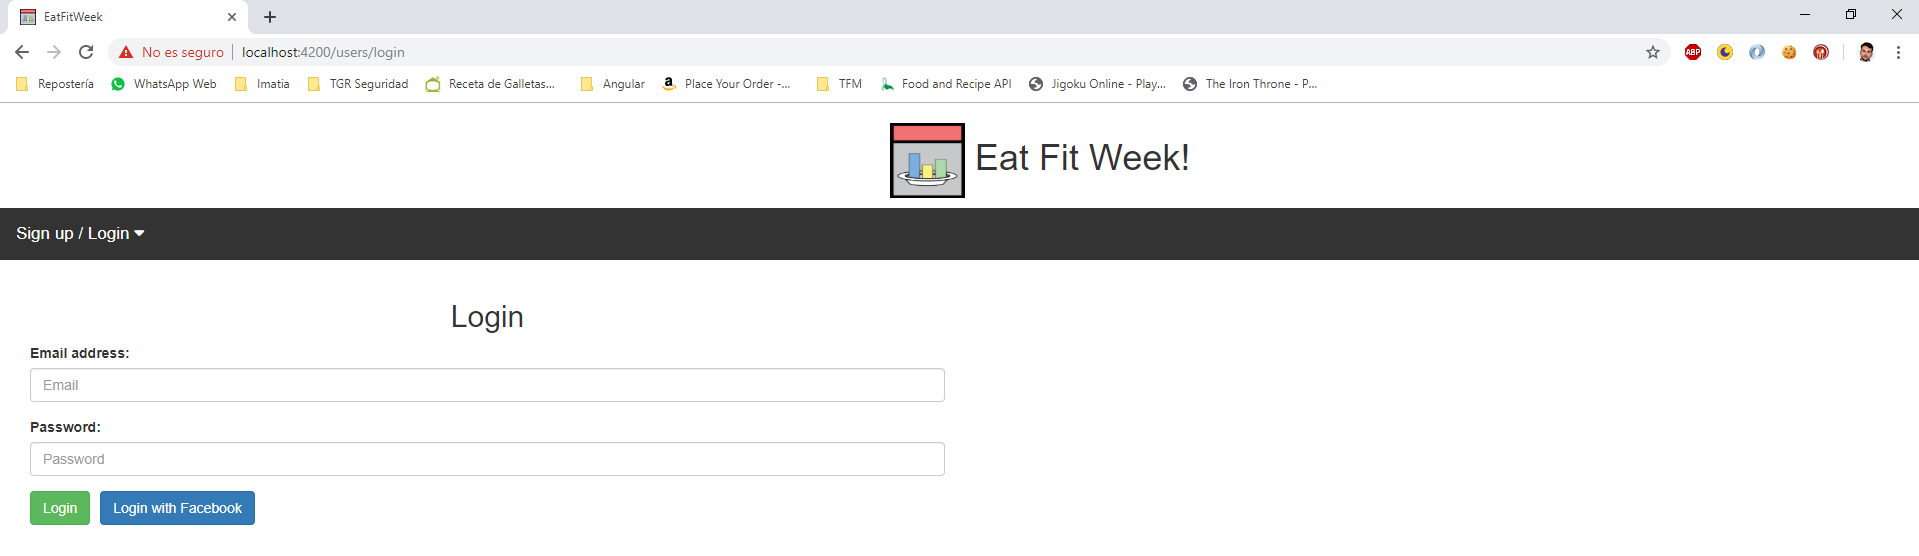
\includegraphics[width=15cm]{Imagenes/MU-Login.png}
		\caption{Log in}\label{Log in}
	\end{figure}
	\subsection{Registro}
	Al presionar en el botón de Registro se muestra el formulario en el que se solicitan los datos necesarios para dar de alta un nuevo usuario: Email, nombre, apellidos y contraseña.\\
	En caso de indicarse datos correctos y confirmar, se creará una nueva cuenta para el usuario y se le redirigirá a la pantalla de inicio de sesión para que pueda autenticarse con la cuenta recién creada.
	\begin{figure}[H]
		\centering
		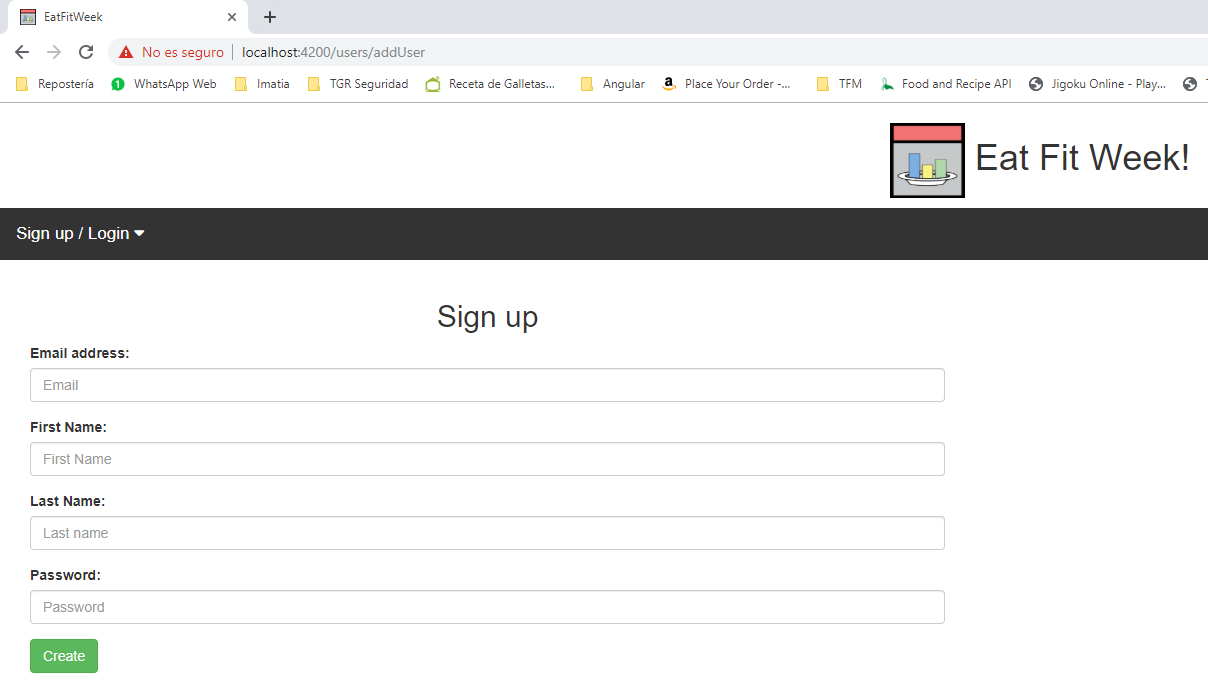
\includegraphics[width=15cm]{Imagenes/MU-Registro.png}
		\caption{Sign up}\label{Sign up}
	\end{figure}
	\subsection{Añadir ingrediente}
	Una vez autenticado, se permite al usuario acceder al resto de funcionalidades de la aplicación. Entre ellas, se encuentra el formulario de añadir ingrediente.\\
	En este formulario se le solicita al usuario: nombre del ingrediente que quiere registrar, su categoría alimenticia y sus stats nutricionales(Calorías, Proteinas, Grasas y Carbohidratos). Una vez rellenado el nombre del ingrediente se le permite al usuario intentar estimar automáticamente los stats nutricionales del ingrediente pulsando en el botón de estimación.
	\begin{figure}[H]
		\centering
		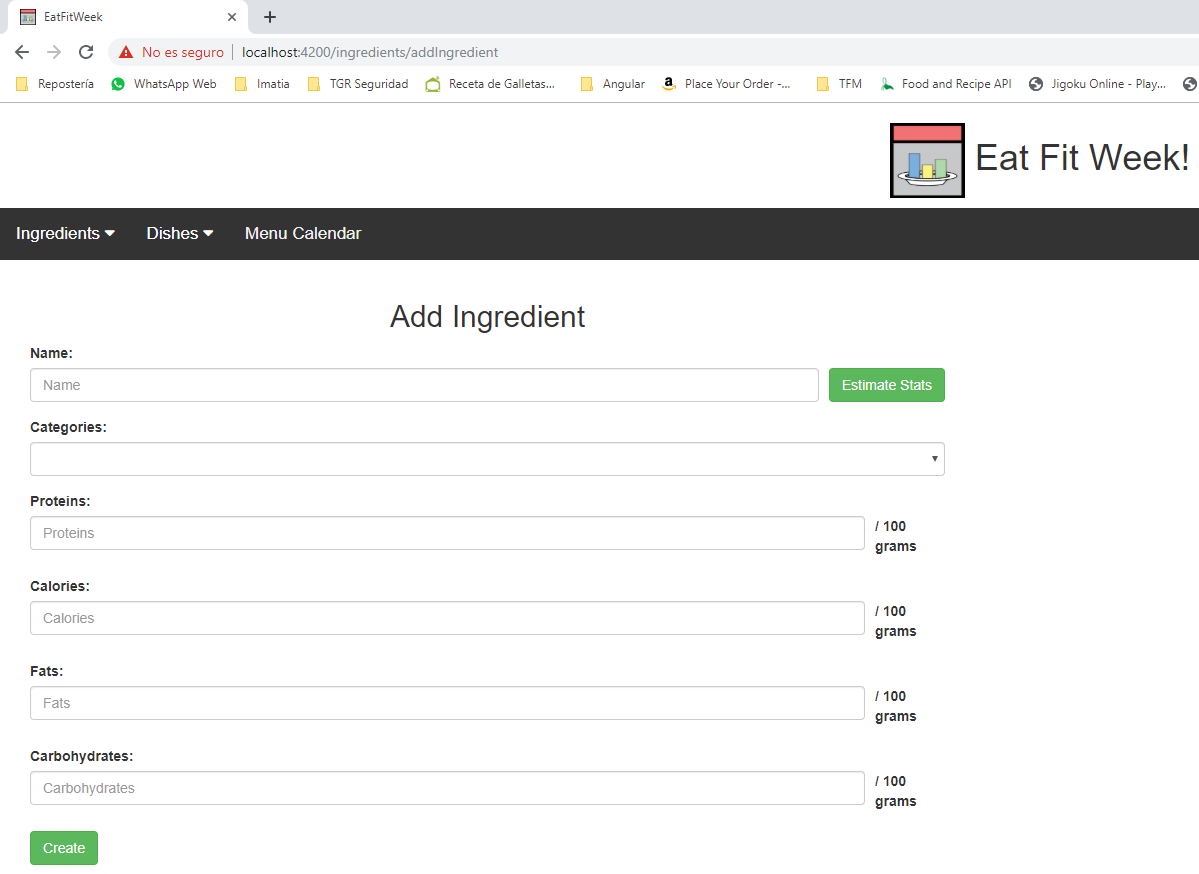
\includegraphics[width=15cm]{Imagenes/MU-AddIngredient.png}
		\caption{Add ingredient}\label{Add ingredient}
	\end{figure}
	\begin{figure}[H]
		\centering
		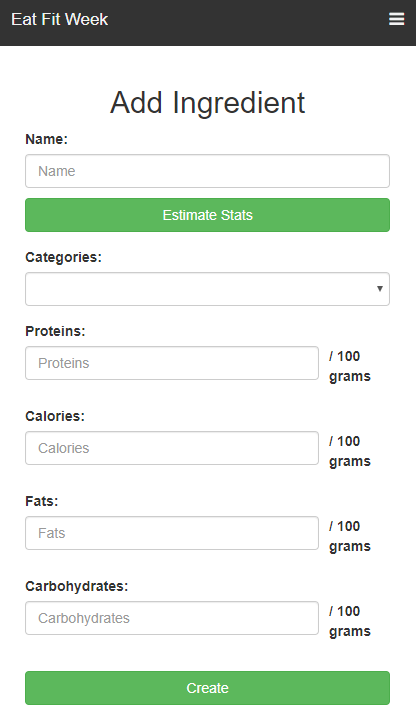
\includegraphics[width=10cm]{Imagenes/MU-AddIngredientMobileTablet.png}
		\caption{Add ingredient Mobile And Tablet}\label{Add ingredient Mobile And Tablet}
	\end{figure}
	\subsection{Listado ingredientes}
	Al seleccionar en el menú ``Listado de ingredientes'' se le permite ver al usuario todos sus ingredientes registrados y, para cada uno de ellos, se visualiza: su nombre, su categoría alimenticia y sus stats nutricionales.\\ También se muestra un warning en caso de que el ingrediente pertenezca a una categoría de las prohibidas por el usuario. Por último, se permite para cada ingrediente acceder a su formulario de actualización o bien borrarlo.\\
	En la versión tablet no se muestra el warning por el escaso espacio en el diseño y en la versión mobile solo se muestran las calorías de los stats nutricionales al ser el stat más relevante.
	\begin{figure}[H]
		\centering
		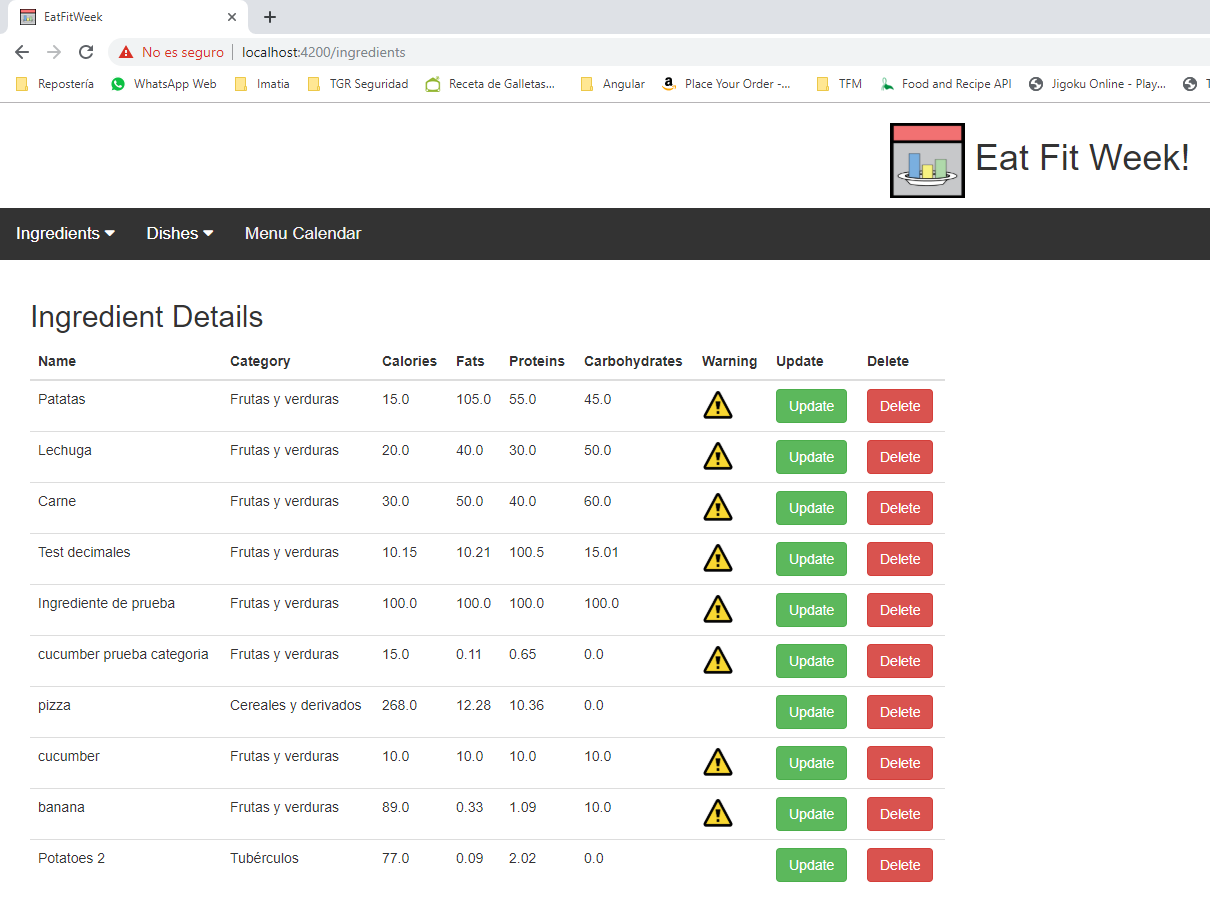
\includegraphics[width=15cm]{Imagenes/MU-ListIngredients.png}
		\caption{List ingredients}\label{List ingredients}
	\end{figure}
	\begin{figure}[H]
		\centering
		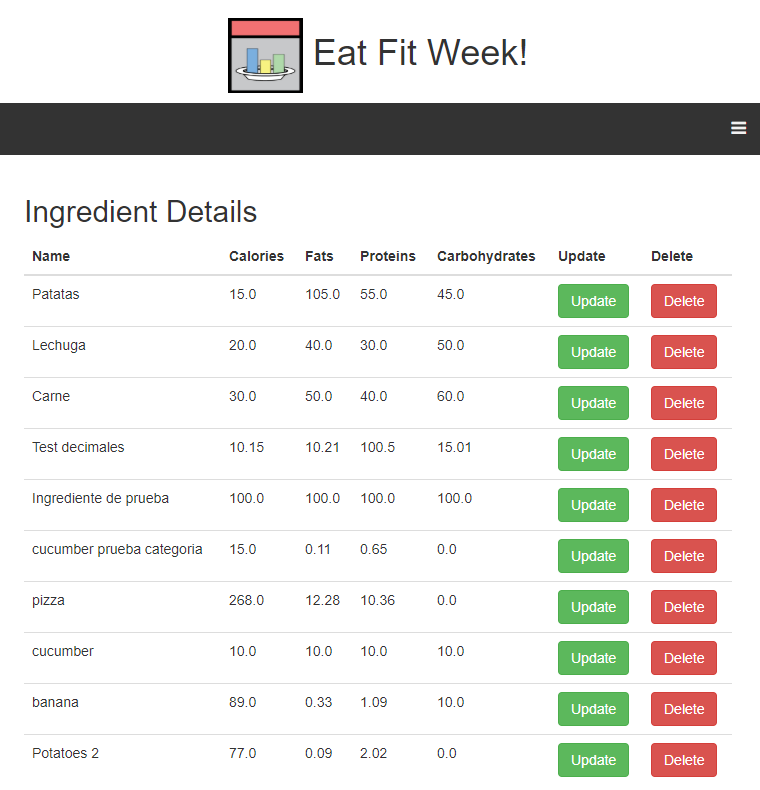
\includegraphics[width=15cm]{Imagenes/MU-ListIngredientsTablet.png}
		\caption{List ingredients Tablet}\label{List ingredients Tablet}
	\end{figure}
	\begin{figure}[H]
		\centering
		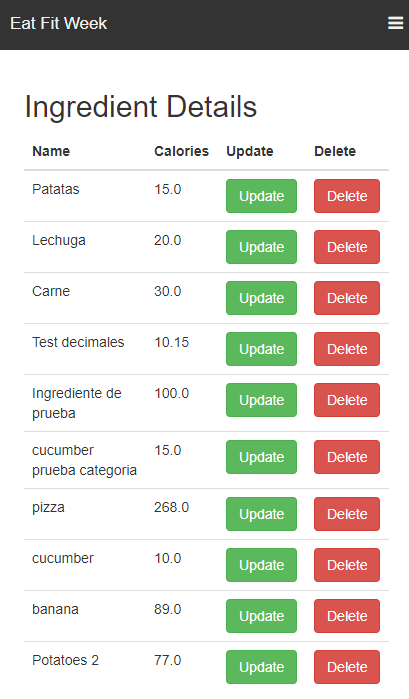
\includegraphics[width=10cm]{Imagenes/MU-ListIngredientsMobile.png}
		\caption{List ingredients Mobile}\label{List ingredients Mobile}
	\end{figure}
	\subsection{Actualización ingrediente}
	Al seleccionar el botón ``Actualizar'' en una de las filas del listado de ingredientes se accede al formulario de actulización de ingrediente. Presenta los mismos campos y misma funcionalidad que el formulario de añadir ingrediente pero se utiliza únicamente sobre ingredientes ya dados de alta y está inicializado con los datos del ingrediente.	
	\begin{figure}[H]
		\centering
		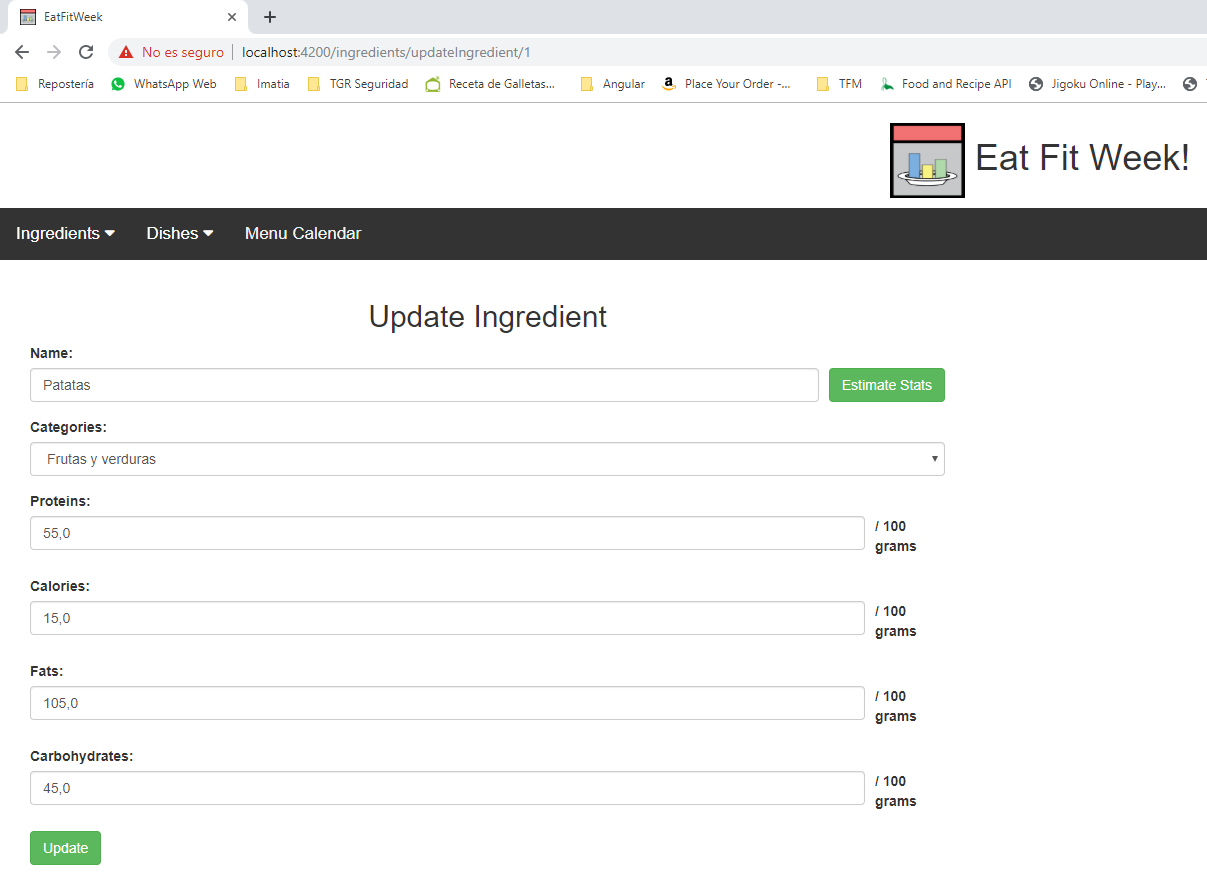
\includegraphics[width=15cm]{Imagenes/MU-UpdateIngredient.png}
		\caption{Update ingredient}\label{Update ingredient}
	\end{figure}
	\begin{figure}[H]
		\centering
		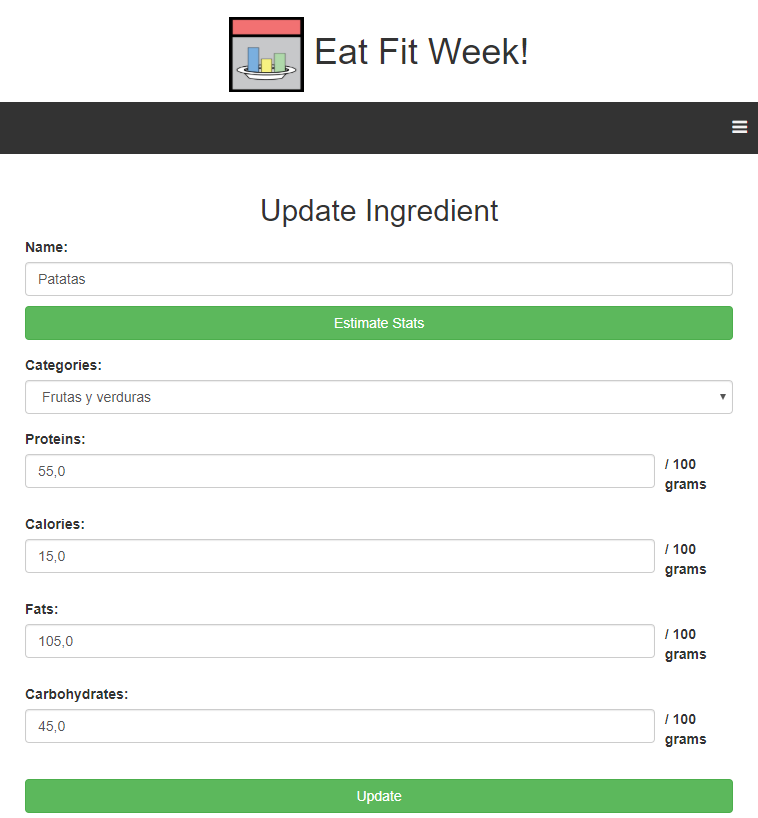
\includegraphics[width=15cm]{Imagenes/MU-UpdateIngredientMobileTablet.png}
		\caption{Update ingredient Mobile Tablet}\label{Update ingredient Mobile And Tablet}
	\end{figure}
	\subsection{Añadir plato}
	Al seleccionar en el menú ``Añadir plato'' se permite acceder a su formulario, en él se le solicita al usuario: los ingredientes que componen el plato y para cada uno de ellos la cantidad del ingrediente en el plato, se le solicita la receta de elaboración del plato, las comidas en las que estará permitido el plato (Inicialmente se permite en todas) y por último el nombre del plato.
	Una vez añadido un ingrediente, se mostrarán tanto los ingredientes que tiene el plato seleccionados como sus stats nutricionales. El campo del nombre del plato tiene un mecanismo de auto rellenado para facilitar la labor del usuario: Con el primer ingrediente seleccionado, se establece como nombre del plato y los siguientes ingredientes seleccionados se añaden al nombre mediante conjunciones, por ejemplo: en caso de seleccionar tres ingredientes en este orden, Carne, Patatas y Lechuga; el nombre del plato se iniciará a ``Carne con Patatas y Lechuga''. De todas formas en todo momento se permite al usuario editar ese nombre por si quiere editarlo o elegir uno propio.
	\begin{figure}[H]
		\centering
		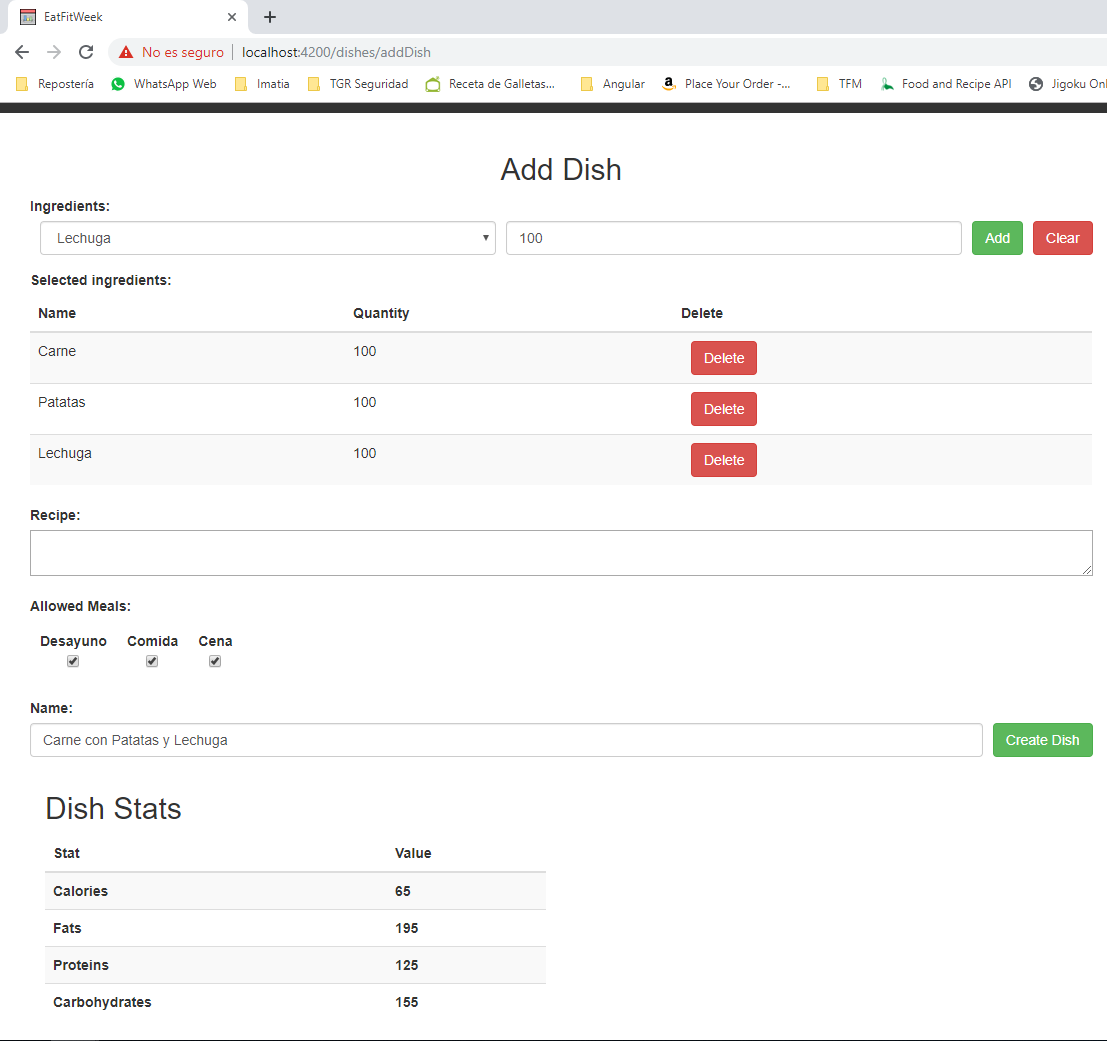
\includegraphics[width=15cm]{Imagenes/MU-AddDish.png}
		\caption{Add dish}\label{Add dish}
	\end{figure}
	\begin{figure}[H]
		\centering
		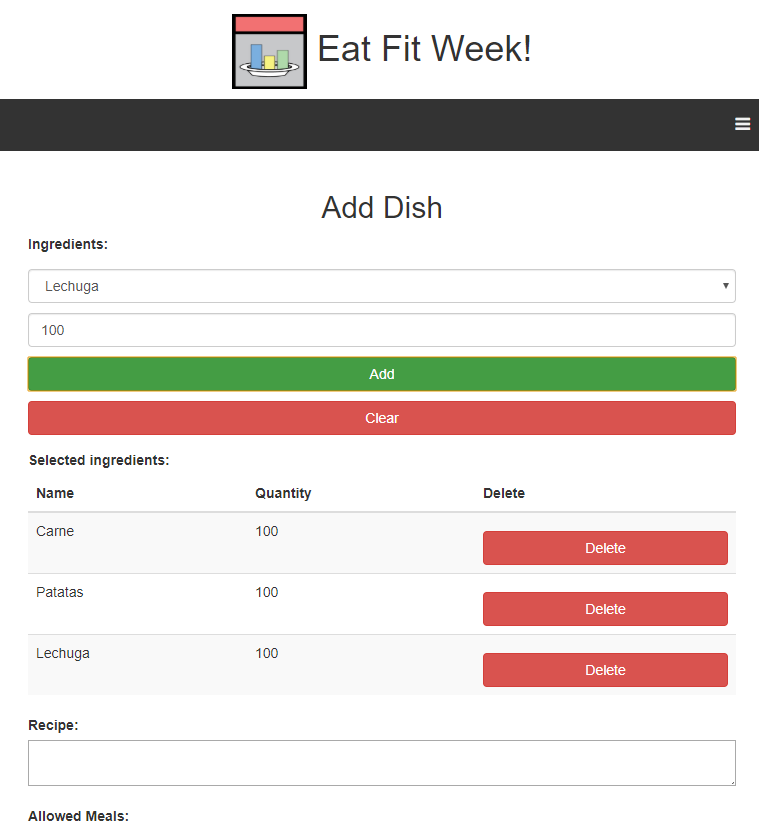
\includegraphics[width=15cm]{Imagenes/MU-AddDishMobileTablet.png}
		\caption{Add dish Mobile And Tablet}\label{Add dish Mobile And Tablet}
	\end{figure}
	\subsection{Listado de platos}
	Al seleccionar en el menú ``Listado de platos'' se accederá a su formulario en el que se visualizarán todos los platos registrados por el usuario. Para cada uno de ellos se visualizarán los siguientes datos: nombre y stats nutricionales. También se permitirá acceder a su actualización, borrar el plato o bien añadirlo al menú actual en el primer hueco válido para el plato.\\
	En la versión tablet no se muestra la opción de añadir el plato al menú actual ya que no tiene tanto sentido al no verse toda la semana en el mismo formulario y poder confundir al usuario y en la versión mobile solo se muestran las calorías de los stats nutricionales al ser el stat más relevante y tener escaso espacio en el diseño.
	\begin{figure}[H]
		\centering
		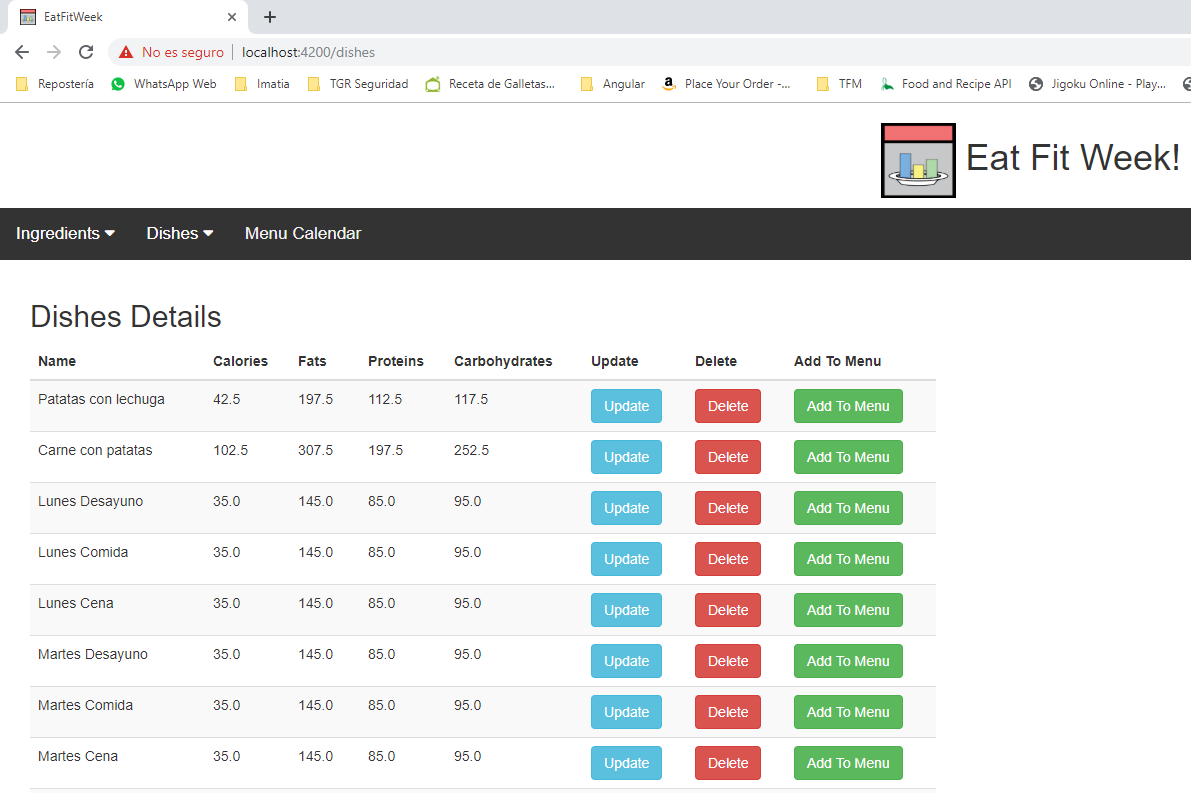
\includegraphics[width=15cm]{Imagenes/MU-ListDishes.png}
		\caption{List dishes}\label{List dishes}
	\end{figure}
	\begin{figure}[H]
		\centering
		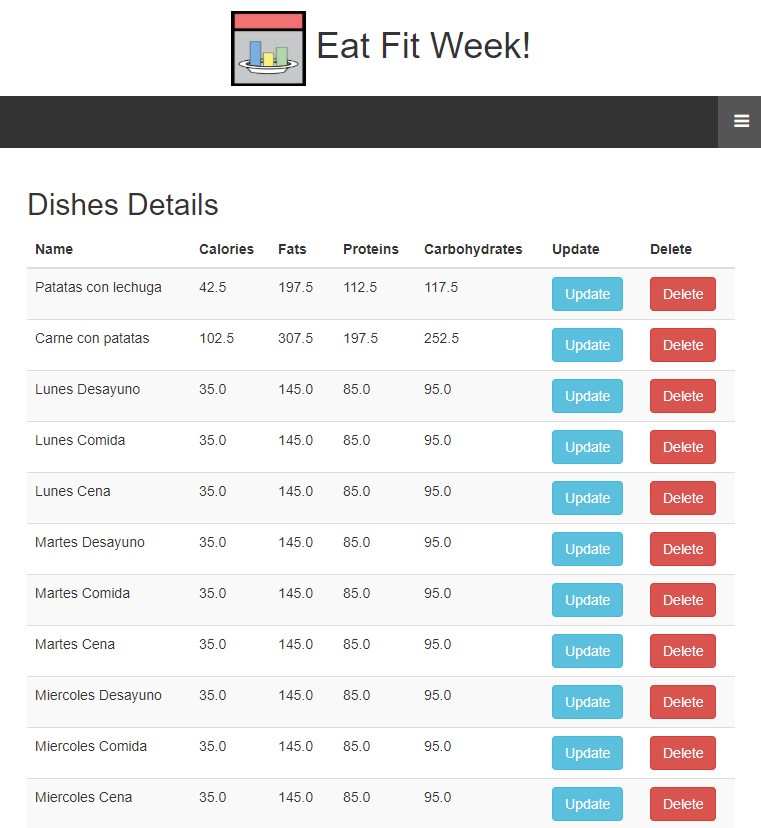
\includegraphics[width=15cm]{Imagenes/MU-ListDishesTablet.png}
		\caption{List dishes Tablet}\label{List dishes Tablet}
	\end{figure}
	\begin{figure}[H]
		\centering
		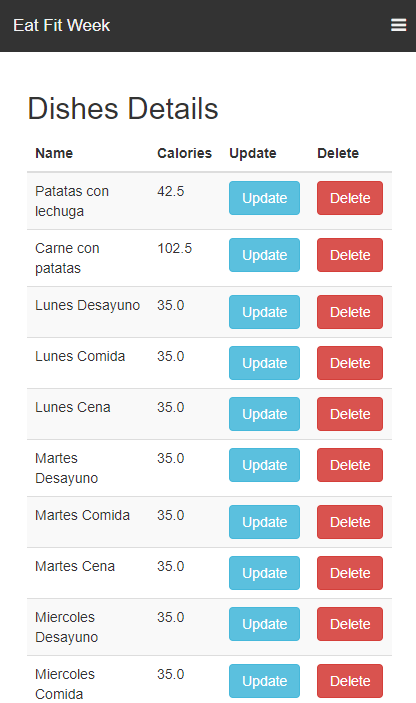
\includegraphics[width=10cm]{Imagenes/MU-ListDishesMobile.png}
		\caption{List dishes Mobile}\label{List dishes Mobile}
	\end{figure}
	\subsection{Actualización de plato}
	Al seleccionar el botón ``Actualizar'' en cada fila de la tabla de visualización de platos, se permitirá acceder al formulario de actualización de platos. Tiene el mismo funcionamiento y visualización que el formulario de añadir platos salvo por el hecho de que sólo se puede acceder a él en platos ya registrados y sus datos se inicializan con la información del plato.
	\begin{figure}[H]
		\centering
		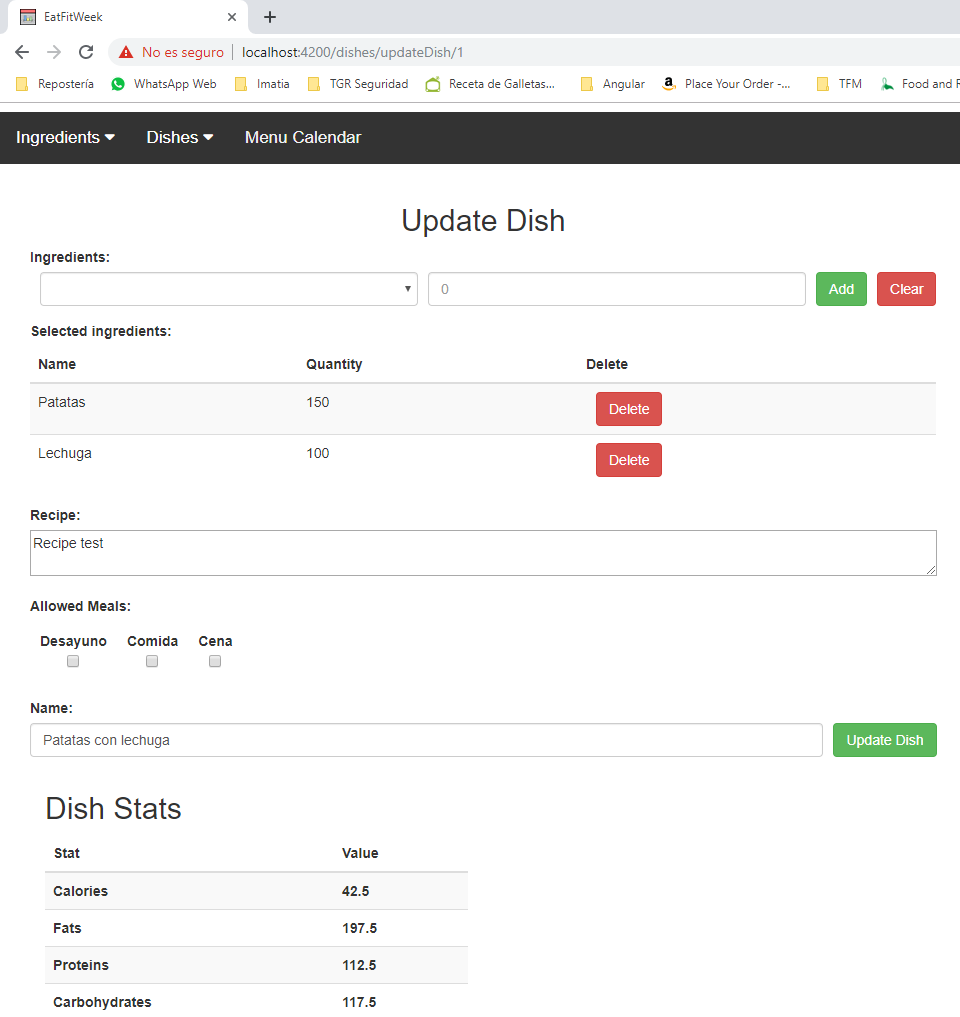
\includegraphics[width=15cm]{Imagenes/MU-UpdateDish.png}
		\caption{Update dish}\label{Update dish}
	\end{figure}
	\begin{figure}[H]
		\centering
		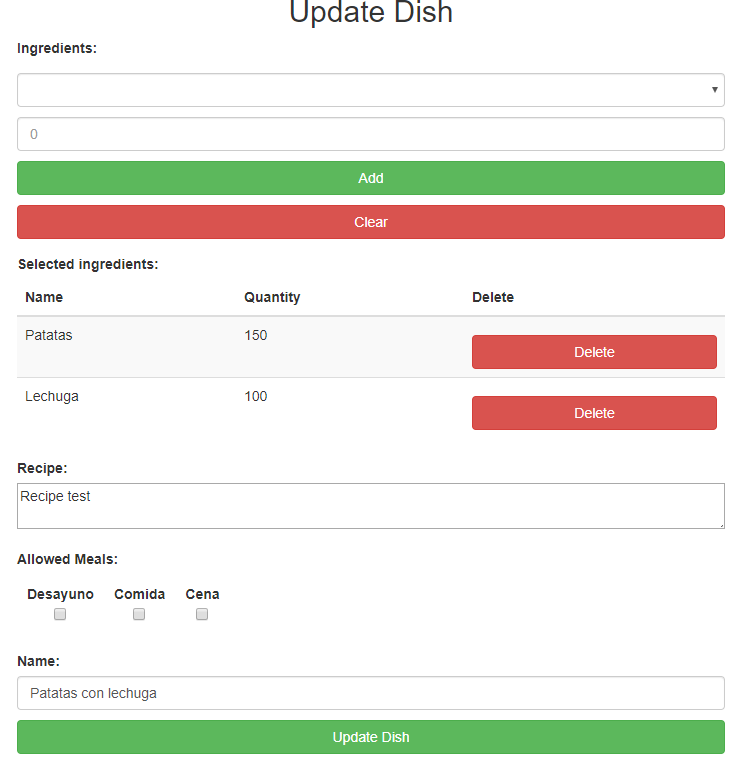
\includegraphics[width=15cm]{Imagenes/MU-UpdateDishMobileTablet.png}
		\caption{Update dish Mobile And Tablet}\label{Update dish Mobile And Tablet}
	\end{figure}
	\subsection{Configuraciones de usuario}
	Al seleccionar ``Configuraciones'' en el menú de usuario conectado se puede acceder a este formulario en el que se permite al usuario configurar el funcionamiento del sistema.\\
	Las configuraciones soportadas son: los valores máximos semanales de los stats nutricionales de los menús, las categorías alimenticias prohibidas por el usuario y las comidas semanales del usuario, tanto su número como su nombre.
	\begin{figure}[H]
		\centering
		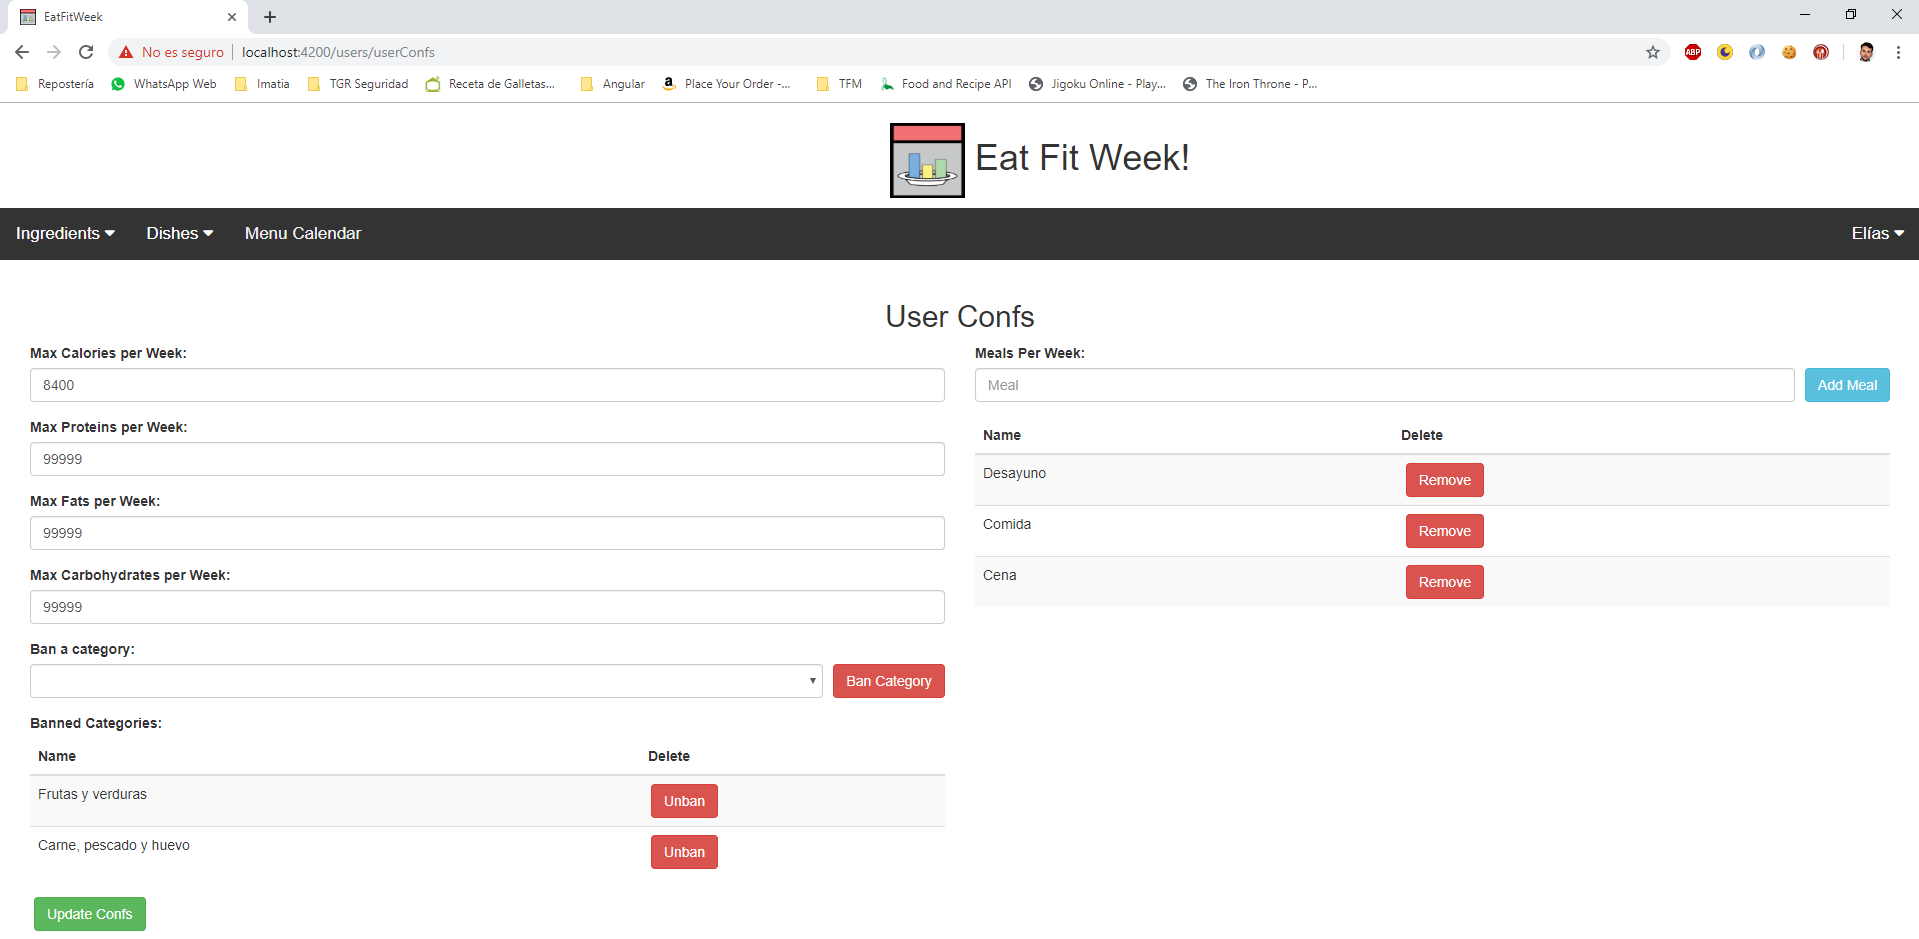
\includegraphics[width=15cm]{Imagenes/MU-UserConfs.png}
		\caption{User configurations}\label{User configurations}
	\end{figure}
	\begin{figure}[H]
		\centering
		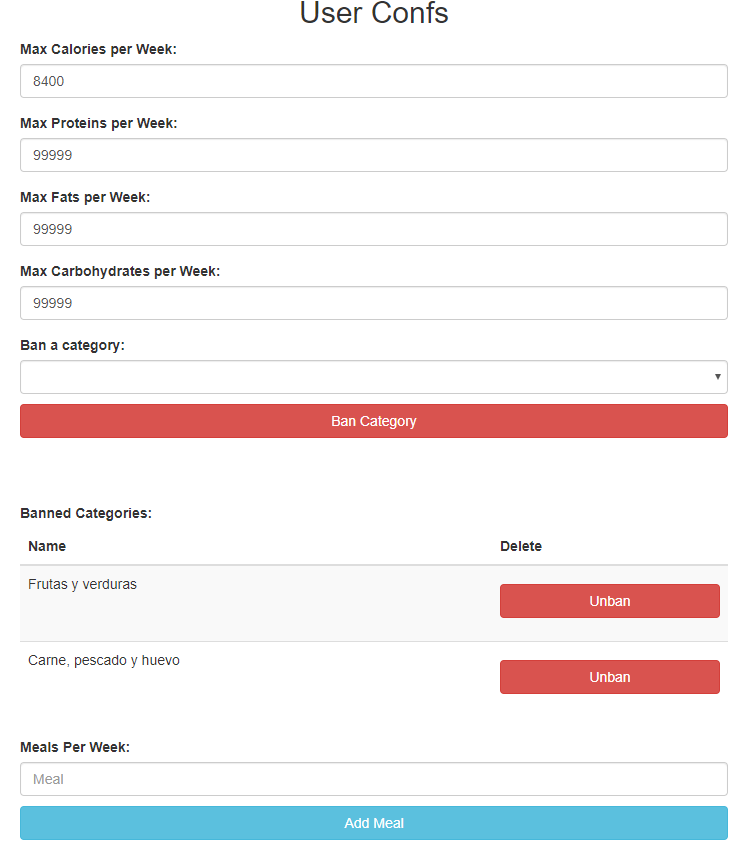
\includegraphics[width=15cm]{Imagenes/MU-UserConfsMobileTablet.png}
		\caption{User configurations Mobile And Tablet}\label{User configurations Mobile And Tablet}
	\end{figure}
	\subsection{Visualización semanal de los menús}
	Al seleccionar ``Calendario de Menú'' en el menú se accede a este formulario que representa la funcionalidad principal del sistema.\\
	Se muestra un grid con cada día de la semana como columnas y con las comidas como filas. Dentro de cada celda del grid, pueden ocurrir dos cosas:
	\begin{itemize}
		\item Que exista un plato planificado para ese hueco concreto del menú actual con lo que se visualizará su nombre. En caso de que el usuario haga click sobre ese hueco, se eliminará el plato del menú. En caso de que se mantenga pulsado ``Shift'' cuando se hace click sobre el plato, se replicará el plato en el menú de forma que se añadirá el mismo plato al siguiente hueco disponible permitido por el plato.
		\item Que no exista un plato para ese hueco concreto del menú actual con lo que se visualizarán dos botones: Uno para añadir un plato de entre los registrados por el usuario en ese hueco seleccionado y otro para  que el sistema sugiera al usuario un plato para ese hueco concreto.
	\end{itemize}
	Inicialmente se mostrará el menú que se corresponda con la semana en la que el usuario está accediendo al sistema pero se le permite desplazarse por semanas anteriores o siguientes sin límite.\\
	Se muestran también los stats nutricionales sumados de todos los platos del menú y se permite modificar la visualización para que se pueda cambiar a visualización diaria y se pueda seleccionar el día concreto del que se quiera visualizar sus stats. En caso de estar visualizándose los stats semanales se mostrará una marca que indique al usuario si se cumple con sus limites semanales o si se están infringiendo.\\
	Para todos los menús se visualizan una serie de acciones posibles, de izquierda a derecha: mostrar su lista de la compra, eliminar los platos del menú, rellenar el menú con platos aleatorios, rellenar el menú con platos que no violen los límites nutricionales del usuario, guardar los platos del menú como una plantilla para cargar en otros menús, rellenar el menú con los platos de una plantilla previamente guardada por el usuario y por último imprimir el menú.
	En la visión tablet se visualizan tres días de cada vez en lugar del menú entero y en la visión mobile se visualiza un día de cada vez.\\
	En estas dos visiones se puede hacer scroll al siguiente tramo o al anterior mediante swipe hacia la izquierda y hacia la derecha respectivamente. Al llegar al final de la semana y hacer swipe hacia la izquierda se visualiza un formulario en el que se ve el resumen del menú semanal, , y se ofrecen las mismas acciones sobre el menú que en la versión standard.
	\begin{figure}[H]
		\centering
		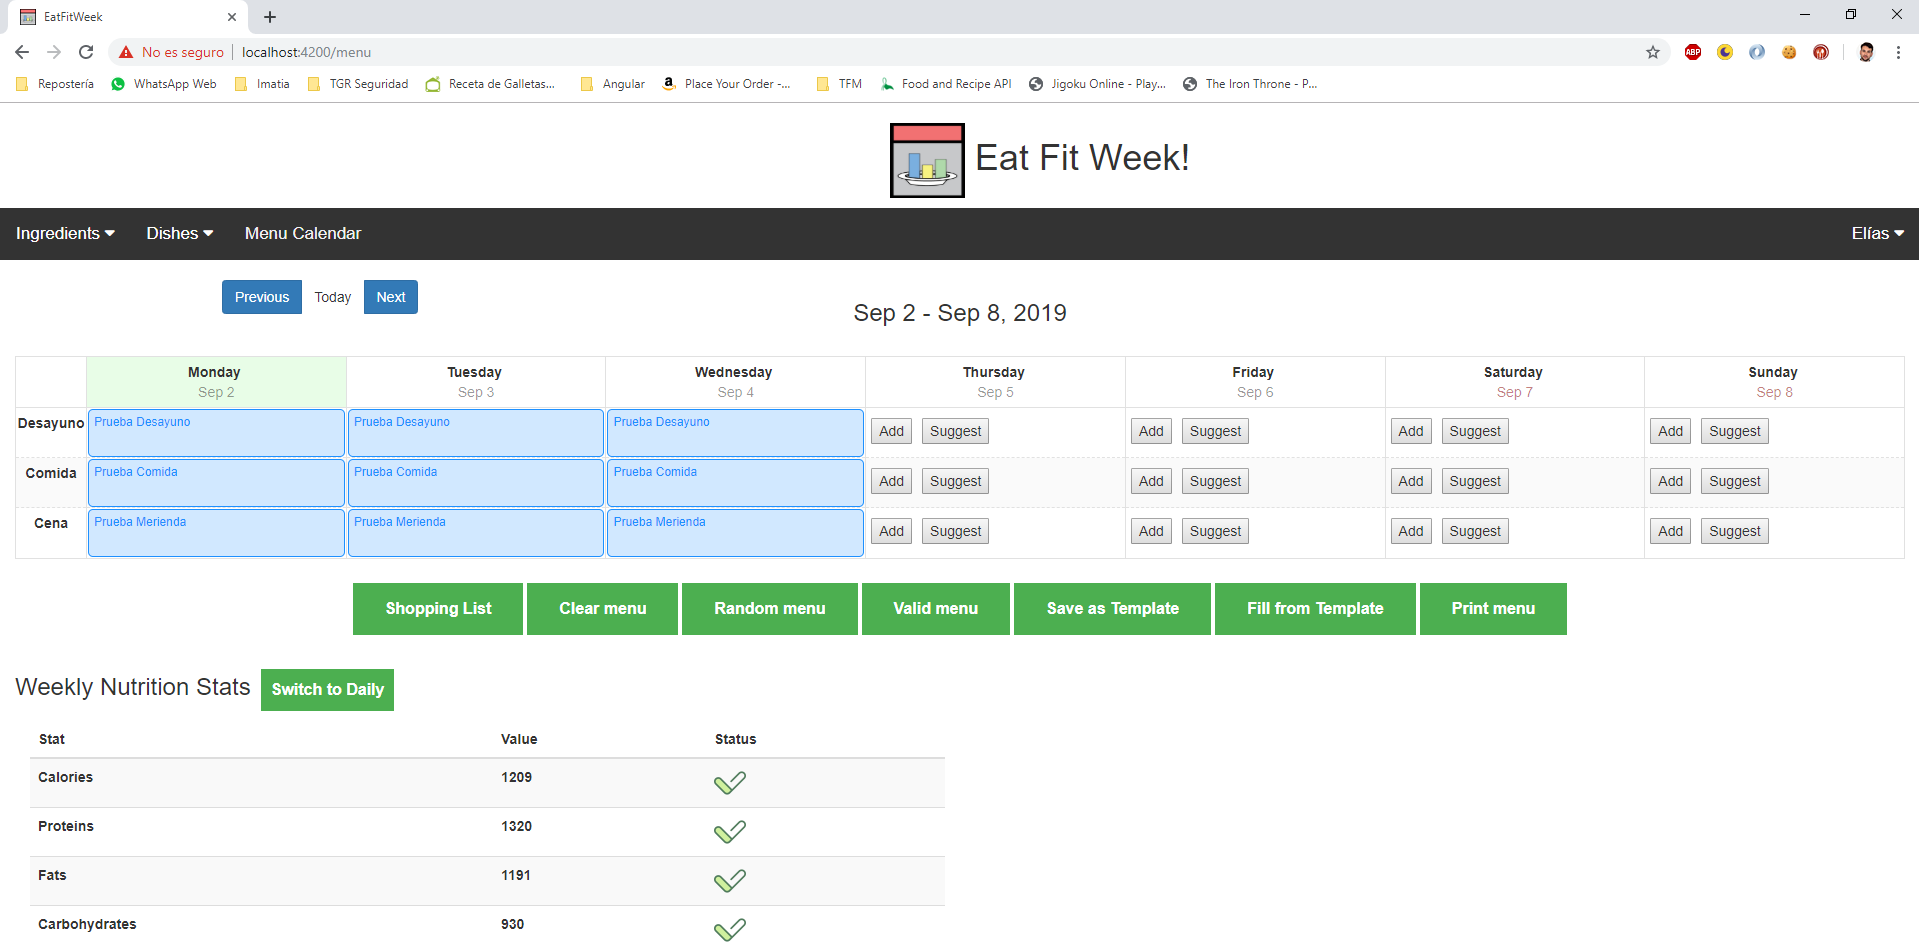
\includegraphics[width=15cm]{Imagenes/MU-MenuView.png}
		\caption{Menu View}\label{Menu View}
	\end{figure}
	\begin{figure}[H]
		\centering
		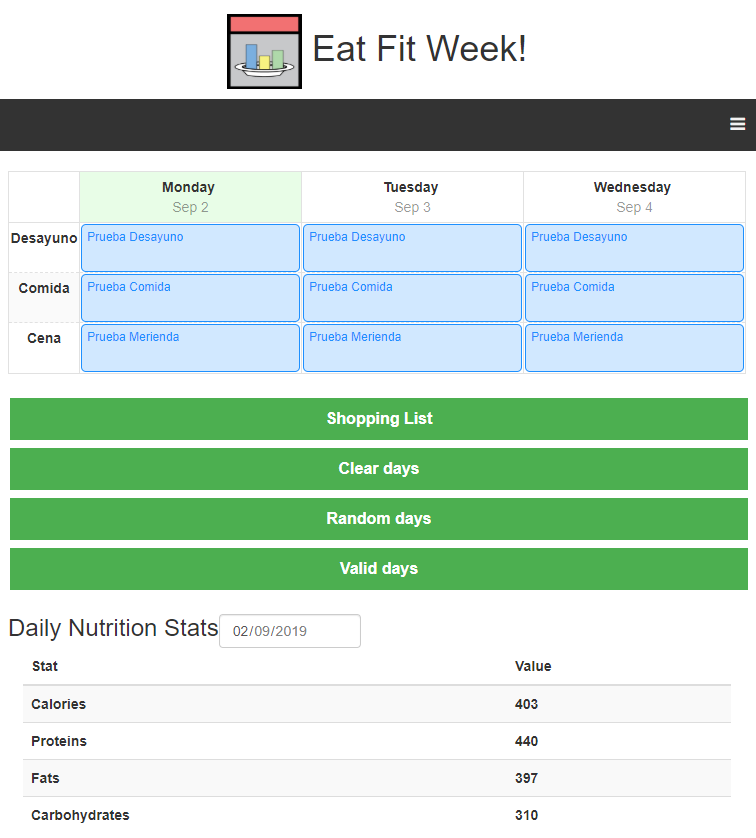
\includegraphics[width=15cm]{Imagenes/MU-MenuViewTablet.png}
		\caption{Menu View Tablet}\label{Menu View Tablet}
	\end{figure}
	\begin{figure}[H]
		\centering
		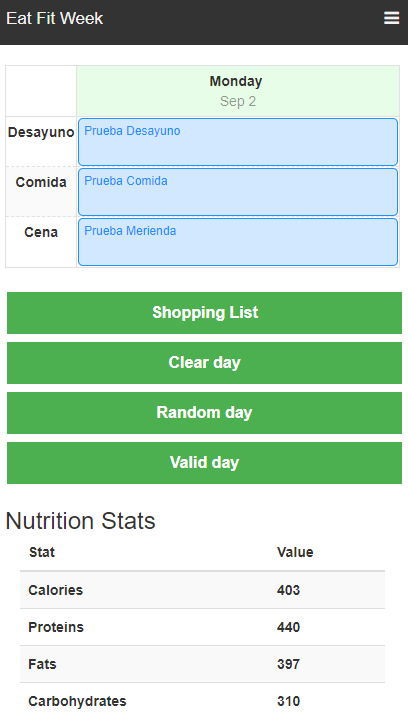
\includegraphics[width=10cm]{Imagenes/MU-MenuViewMobile.png}
		\caption{Menu View Mobile}\label{Menu View Mobile}
	\end{figure}
	\begin{figure}[H]
		\centering
		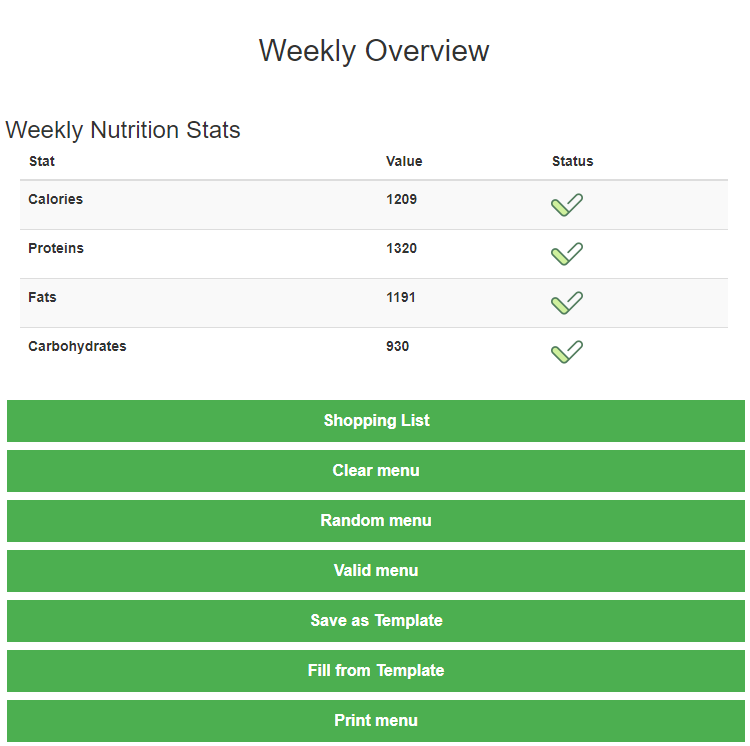
\includegraphics[width=15cm]{Imagenes/MU-MenuWeekViewMobileTablet.png}
		\caption{Menu Week View Mobile And Tablet}\label{Menu Week View Mobile And Tablet}
	\end{figure}
	
\end{document}

